\documentclass[UTF8, 10pt, a4paper, oneside]{ctexart}
\usepackage{amsmath}
\usepackage{amsthm}
\usepackage{amsfonts}
\usepackage{amssymb}
\usepackage{amstext}
\usepackage[version=4]{mhchem}
\usepackage{geometry}
\usepackage{changepage}
\usepackage{paralist}
\usepackage{graphicx}
\usepackage{extarrows}
\usepackage{xcolor}
\geometry{left=1.27cm, right=1.27cm, top=1.27cm, bottom=1.5cm}
\linespread{1.5}
\title{\vspace{-2em} 高考模拟卷 \vspace{-1em}}
\author{盛炯元 \quad 杨元谦}
\date{\textcolor{white}{\today}\vspace{-3em}}
\pagestyle{plain}

\newcommand{\blank}{ \underbar{\quad$\blacktriangle$\quad} }% 空格样式
\newcommand{\fs}[1]{{\fangsong #1}}% 使用仿宋
\newcommand{\circled}[1]{{\small{\textcircled{\tiny{#1}}}}}% 圈圈数字
\newcommand{\Romannumeral}[1]{\uppercase\expandafter{\romannumeral#1}}% 大写罗马数字
\newcommand{\chdots}{…\hspace{-0.15em}…}% 中文省略号调教

\theoremstyle{definition}
\newtheorem{exercise}{}
\newtheorem{subexercise}{}[exercise]% 用于兼容编号错误或是内含的高考题等

\theoremstyle{remark}
\newtheorem*{answer}{【答案】}
\newtheorem*{point}{【考点】}      % 考点&易错点
\newtheorem*{method}{【方法】}     %(可选)
\newtheorem*{explanation}{【解析】}     %

\theoremstyle{plain}
\newtheorem*{note}{【注】}  %(可选)

\begin{document}
\maketitle

\begin{exercise}
蛋白质是结构和功能多样的生物大分子,下列叙述正确的是\quad(\quad)
\begin{adjustwidth}{2em}{}
        \begin{asparaenum}[A. ]
            \item 二硫键的断裂不会改变蛋白质的空间结构
            \item 血浆里,人体三大供能物质中质量分数最大的是蛋白质
            \item 向蛋白质溶液中加入浓的硫酸铜溶液可使蛋白质发生盐析
            \item 利用基因工程可以“创造”出自然界中原先不存在的蛋白质
        \end{asparaenum}
\end{adjustwidth}
\begin{answer}
    B
\end{answer}
\begin{point}
    蛋白质空间结构、血液中糖脂蛋相对含量、盐析与变性、基因工程局限性
\end{point}
\begin{explanation}
    二硫键影响蛋白质的三、四级结构,进而影响其整体空间结构,A选项错误;血浆中水占91\%$\sim$92\%,蛋白质约占7\%\textsuperscript{\fs{[义务教育教科书·生物学七年级下册 P35]}},B选项正确;铜离子是重金属,会使蛋白质发生变性,而不是盐析,C选项错误;基因工程原则上只能生产自然界中已存在的蛋白质,D选项错误。
\end{explanation}
\end{exercise}

\begin{exercise}    
在一定温度下,大田的某种植物绿色叶片的光合速率和呼吸速率的平均对光照强度的响应曲线如图所示。下列说法错误的是\quad(\quad)
\begin{adjustwidth}{2em}{}\vspace{-2em}
    \begin{figure}[h!]
        \flushright
        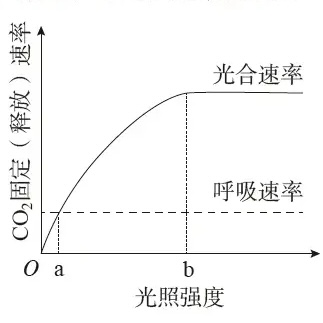
\includegraphics[width=0.3\textwidth]{assists/2-1.jpg}
    \end{figure}\vspace{-16em}
        \begin{asparaenum}[A. ]
            \item 生长于光照强度为a环境的植株生长最将因匮乏营养而死亡
            \item 光照强度从a逐渐增加到b时,该植物生长速率逐渐增大
            \item 光照强度小于b时,提高大田$\ce{CO2}$浓度,$\ce{CO2}$固定速率会增大
            \item 光照强度为b时,适当降低光反应速率,$\ce{CO2}$固定速率会降低
        \end{asparaenum}
\end{adjustwidth}
\begin{answer}
    C
\end{answer}
\begin{point}
    总光合速率、净光合速率
\end{point}
\begin{explanation}
    生长于光照强度为a环境的植株虽然其叶片的总光合速率与呼吸速率相等,但植株中总有无法进行光合作用的组织(如根、花、果实)消耗着贮存的有机物,A选项正确;光照强度小于b时,影响光合作用的主要因素为光照,提高大田$\ce{CO2}$浓度不一定使$\ce{CO2}$固定速率增大,C选项错误。
\end{explanation}
\end{exercise}

\end{document}